\documentclass[10pt]{article}
\usepackage[a4paper,left=2.54cm,top=2.54cm,right=2.54cm,bottom=2.54cm]{geometry}
\usepackage{fancyhdr}
\setlength{\headsep}{1.cm} % Adjust the space after the header
\usepackage{afterpage}
\usepackage{setspace}
\usepackage{bibspacing}
\usepackage{float}
\singlespacing

%%%% YOU CAN PUT YOUR OWN DEFINITIONS HERE
\newfont{\toto}{msbm10 at 12 pt}
\newfont{\ithd}{cmr9}
\newcommand{\equa}[1]{(\ref{eq:#1})}
\newcommand{\laeq}[1]{\label{eq:#1}}
\newcommand{\figu}[1]{\ref{fig:#1}} 
\newcommand{\lafi}[1]{\label{fig:#1}}
\newcommand{\fmo}{\tilde{U}}
\newcommand{\fve}{\tilde{u}}
\newcommand{\Dt}{\Delta t}

\newcommand{\R}{\mathbb{R}}
\newcommand{\Z}{\mathbb{Z}}
\newcommand{\si}[1]{\rm\scriptscriptstyle{#1}}
%%%% END OF YOUR DEFINITIONS 

\pagestyle{fancyplain}
\renewcommand{\headrulewidth}{0pt}

\usepackage{amsmath,amsthm,amsfonts,amssymb}
\usepackage{physics}
\usepackage[pdftex]{graphicx}
\usepackage[T1]{fontenc}

%%%% CONFERENCE HEADER. REPLACE xxxx WITH 4-DIGIT PAPER NUMBER ASSIGNED BY CONFERENCE COMMITTEE.

\rhead{\ithd{\bf ICCFD12-2024-xxxx\\  \   \\}}
\lhead{\ithd{\bf Twelfth International Conference on \\      
Computational Fluid Dynamics (ICCFD12), \\
Kobe, Japan, July 14-19, 2024
}}


\usepackage{titling}
\setlength{\droptitle}{0em}  
\pretitle{\vspace{-4em}\begin{center}\LARGE}
\posttitle{\end{center}\vspace{-1em}}
\preauthor{\begin{center}\large}
\postauthor{\end{center}\vspace{-6em}}


\title{
\bf A Novel Energy-based Artificial Viscosity for Suppressing Numerical Oscillations in Discontinuous Galerkin and Flux Reconstruction Schemes
}
\author{
Weicheng Pei$^{*}$ and Yu-Xin Ren$^{*}$\\
Corresponding author: weicheng.pei@icloud.com\\
$^{*}$ Department of Engineering Mechanics, Tsinghua University, Beijing 100084, China
}
\date{}

\usepackage[colorlinks=true]{hyperref}
\usepackage[]{physics}

\begin{document}

%%%% TITLE
\maketitle
\afterpage{\fancyhead{}}

%%%% ABSTRACT AND KEYWORDS
%\vskip0.5cm
\centerline{
}
\vskip0.5cm 

%%%% MAIN PART
\section{Introduction}
To construct high-order schemes on unstructured meshes, the discontinuous Galerkin (DG) method \cite{Cockburn_2001,Hesthaven_2008} and the flux reconstruction (FR) method \cite{Huynh_2007,Huynh_2014} are two of the most popular choices in the community of computational fluid dynamics (CFD).
%
Besides the inherent compactness, these schemes are much easier to implement $p$-refinement than their finite difference and finite volume counterparts.
%
However, like other high-order schemes, numerical oscillations would appear near discontinuities or large gradients in the solution given by a DG or FR scheme, if no shock fitting or shock capturing mechanism were incorporated into it.
%

%
Various shock capturing techniques, such as limiters \cite{Zhong_2013,Zhu_2013,Zhu_2020,Zhu_2023,Li_2020}, filters \cite{Panourgias_2016,Dzanic_2022} and artificial viscosities \cite{Persson_2006,Klockner_2011,Discacciati_2020}, have been developed for DG and FR schemes in the past two decades.
%
However, most of these methods are based on orthogonal (modal) expansions, which are less efficient than pure Lagrange (nodal) expansions.
%
Some of them are even built upon extrapolations, i.e. evaluating an approximating polynomial outside the element it belongs to, which impairs the compactness of DG and FR schemes.
%

%
In this paper, a novel artificial viscosity based on an energy measure of oscillation and its damping rate on a DG or FR element is developed.
%
The oscillation energy, which measures the amplitude of numerical oscillations on a given element, is obtained by evaluating the $L_2$-norm of the difference between the numerical solutions on the element and its neighbors.
%
The damping rate of this energy on an element can be derived under the assumptions of linear flux--gradient relation and constant viscosity distribution.
%
The value of viscosity for suppressing numerical oscillations is obtained by taking the ratio of the oscillation energy with respect to the product of its damping rate and prescribed time step.
%
Such element-wise constant viscosity distribution could optionally be reconstructed to be $C_0$ continuous on element interfaces.

\section{Methodology}
\subsection{Element-wise Polynomial Approximations}
To solve the two-dimensional conservation law
$$
\partial_{t}\,u+\partial_{\vec{r}}\vdot\vec{f}=0,\quad\partial_{\vec{r}}\vdot\vec{f}=\partial_{x}\,f^{x}+\partial_{y}\,f^{y},
$$
using a DG or FR scheme, one may first introduce a map from the physical coordinates to the parametric coordinates on each element:
$$
\underbrace{(x,y)}_{\vec{r}}\mapsto\underbrace{(\xi,\eta)}_{\vec{\rho}}
\implies
\begin{bmatrix}\partial_{\xi}\,\phi\\
\partial_{\eta}\,\phi
\end{bmatrix}=\underbrace{\begin{bmatrix}\partial_{\xi}\,x & \partial_{\xi}\,y\\
\partial_{\eta}\,x & \partial_{\eta}\,y
\end{bmatrix}}_{\underline{J}}\begin{bmatrix}\partial_{x}\,\phi\\
\partial_{y}\,\phi
\end{bmatrix}=\begin{bmatrix}\partial_{\xi}\,\vec{r}\\
\partial_{\eta}\,\vec{r}
\end{bmatrix}\vdot\partial_{\vec{r}}\,\phi,
$$
in which $\underline{J}$ is the Jacobian matrix of the coordinate map.
%
The conservation law in physical coordinates is then (optionally) transformed into the form in parametric coordinates:
$$
\partial_{t}\,U+\partial_{\vec{\rho}}\vdot\vec{F}=0,\quad\partial_{\vec{\rho}}\vdot\vec{F}=\partial_{\xi}\,F^{\xi}+\partial_{\eta}\,F^{\eta},
$$
in which
$$
U=u\,\underbrace{\det(\underline{J})}_{J},\quad\begin{bmatrix}F^{\xi}\\
F^{\eta}
\end{bmatrix}=J\,\underbrace{\begin{bmatrix}\partial_{x}\,\xi & \partial_{y}\,\xi\\
\partial_{x}\,\eta & \partial_{y}\,\eta
\end{bmatrix}}_{\underline{J}^{-1}}\begin{bmatrix}f^{x}\\
f^{y}
\end{bmatrix}=J\begin{bmatrix}\partial_{\vec{r}}\,\xi\\
\partial_{\vec{r}}\,\eta
\end{bmatrix}\vdot\vec{f}.
$$

To obtain an element-wise polynomial approximation of the solution, an orthonormal (modal) expansion or a Lagrange interpolation has to be introduced for $u$ or $U\equiv Ju$ on the $j$th element:
$$
u(\vec{r},t)\approx u_{j}^{h}(\vec{r},t)=\begin{cases}
\sum_{n=1}^{N}\hat{u}_{j,n}(t)\,\phi_{j,n}(\vec{\rho}), & \text{Lagrange interpolation},\\
\sum_{m=1}^{M}\tilde{u}_{j,m}(t)\,\psi_{j,m}(\vec{r}), & \text{orthonormal expansion},
\end{cases}
$$
in which $\phi_{j,n}$ is the Lagrange basis associated with the $n$th node (a.k.a. solution point) on the $j$th element, which satisfies the Kronecker delta property
$$
\phi_{j,m}(\vec{\rho}_{j,n})=\delta_{mn},\quad\forall (m,n)\in\{1,\dots,N\}^2,
$$
while $\psi_{j,m}$ is the $m$th orthonormal basis on the $j$th element, which satisfies the innerproduct delta property
$$
\langle\psi_{j,m}\vert\psi_{j,n}\rangle=\delta_{mn},\quad\forall (m,n)\in\{1,\dots,M\}^2.
$$
%
The coefficient $\hat{u}_{j,n}$ is the nodal value of the approximate solution, i.e. $\hat{u}_{j,n}=u_j^h(\vec{r}(\vec{\rho}_n), t)$,
while the coefficient $\tilde{u}_{j,m}$ is the projection of the approximate solution on the $m$th basis, i.e. $\tilde{u}_{j,m}=\ip{u_j^h}{\psi_{j,m}}$

The number of terms $N$ or $M$ in the summations, i.e. the dimension of the polynomial space, depends on the degree of solution $P$ and the dimension of physical space $D$.
%
For tensor-product elements, e.g. quadrangles, hexahedra, the dimension of a Lagrange basis is equal to the product of the number of solution points in each dimension, which leads to
$$
N(P,D)=(P+1)^D,
$$
%
For building the orthonormal basis (in physical coordinates), one usually apply the Gram--Schmidt process to the basis formed by monomials whose degrees are less than or equal to $P$, which leads to
$$
M(P,D)=\binom{P+D}{D}.
$$
%
In general, the dimension of a nodal basis is much larger than that of the modal basis with the same $(P,D)$.

\subsection{Semi-discretized Systems from DG and FR}
An ordinary differential equation (ODE) system can then be derived from either the DG method or the FR method.
%

%
The DG method requires the conservation law to be satisfied in a weaker sense
$$
\int_{E_j}\phi_n\pdv{u}{t}
=\int_{E_j}\vec{f}\vdot\grad\phi_n
-\oint_{\partial E_j}\vec{\nu}\vdot\vec{f}\,\phi_n,\quad \forall n\in\{1,\dots,N\},
$$
in which the surface integral comes from integration-by-part.
%
The solution $u$ and the flux $\vec{f}$ in the volume integrals should be replaces by one of the polynomial expansion discussed in the previous section,
while the normal component of the flux in the surface integral should be replaced by a common flux function $f^{I}$.
%
This procedure could also be applied to the conservation law in parametric coordinates, which gives
$$
\int_{\mathcal{E}_j}\phi_{n}\pdv{U_j^{h}}{t}=\int_{\mathcal{E}_j}\vec{F}_j^{D}\vdot\grad\phi_{n}-\oint_{\partial\mathcal{E}_j}F^{I}\,\phi_{n},\quad\forall n\in\{1,\dots,N\},
$$
where $\mathcal{E}_j$ represents the \emph{standard} element defined in the parametric space.
%
The superscript $D$ in $\vec{F}_j^{D}$ emphasizes that the approximated flux are discontinuous on element interfaces.
%
Either of the two weak forms gives a semi-discretized ordinary differential equation (ODE) system.

%
The FR method, on the other hand, gives the ODE system by first introducing a $(P+1)$-degree correction function to the discontinuities flux $\vec{F}_j^{D}$, which then becomes $C_0$ continuous on element interfaces.
%
For one-dimensional problems, the correction procedure is given by
$$
F_j^{R}(\xi)=F_j^{D}(\xi) + \qty[F^{I}-F_j^{D}]_{\xi=-1} g_{-1}(\xi) + \qty[F^{I}-F_j^{D}]_{\xi=+1} g_{+1}(\xi),
$$
where the $(P+1)$-degree $g$'s must satisfy
$$
g_{+1}(+1)=1,\quad
g_{+1}(-1)=0,\quad
g_{-1}(-\xi)=g_{+1}(+\xi),\quad \forall\xi\in[-1,1],
$$
and approximate $0$ in some appropriate sense.
Possible choices of $g$ are plotted in Figure \ref{fr:lumping}.
%
\begin{figure}[H]
  \centering
  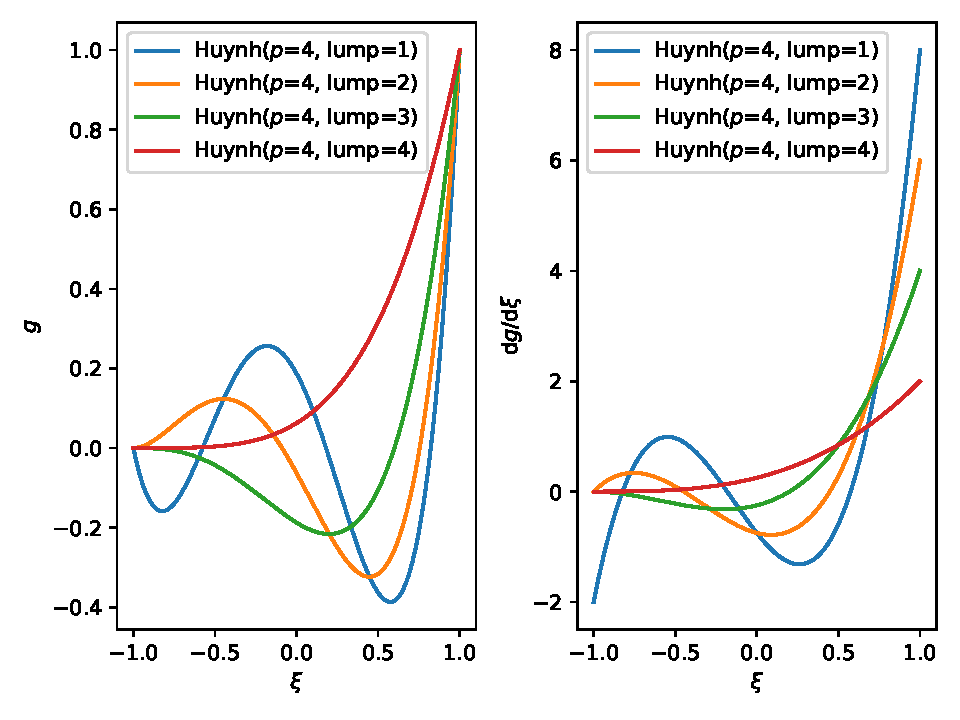
\includegraphics[width=.8\textwidth]{./fr/HuynhLumping.pdf}
  \caption{Candidates of the correction function $g_{+1}$.}
  \label{fr:lumping}
\end{figure}
%
The effect of the correction procedure for the linear convection flux $f(u)=u$ is demonstrated in Figure \ref{fr:compare}.
\begin{figure}[H]
  \centering
  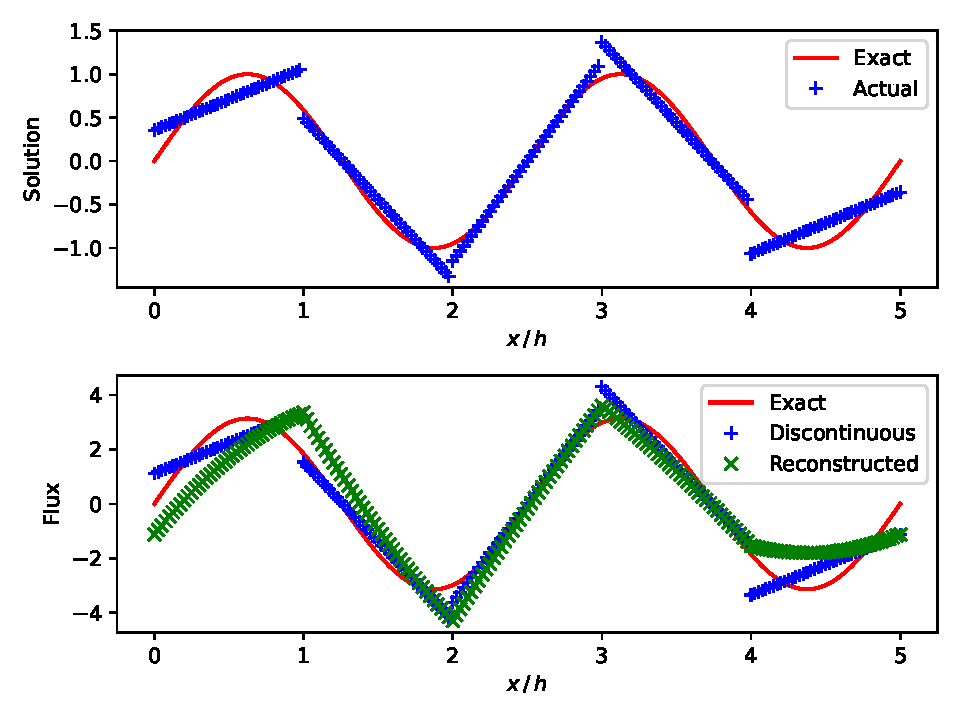
\includegraphics[width=.8\textwidth]{./fr/FRonLegendreRoots.pdf}
  \caption{Discontinuous flux v. reconstructed continuous flux.}
  \label{fr:compare}
\end{figure}

%
By forcing the conservation law to be satisfied on all solution points, and replace $U$ and $F$ by $U_j^h$ and $F_j^{R}$:
$$
\dv{\hat{U}_{j,n}(t)}{t}+\pdv{F_j^{R}(U^{h}(\xi_{n},t))}{\xi}=0,\quad\forall n\in\left\{ 1,\dots,N\right\}.
$$
%
For two-dimensional problems, if the element $E_j$ is a quadrangle, the correction procedure could be applied in a dimension-by-dimension way, which gives
$$
\begin{aligned}\dv{\hat{U}_{j,m,n}}{t} & =\frac{\partial F_{j}^{\xi,D}(\xi_{m},\eta_{n})}{\partial\xi}+\sum_{a=\pm1}\left[F^{I}-F_{j}^{\xi,D}\right]_{\xi=a,\eta_{n}}\dv{g_{a}(\xi_{m})}{\xi}\\
 & +\frac{\partial F_{j}^{\eta,D}(\xi_{m},\eta_{n})}{\partial\eta}+\sum_{b=\pm1}\left[F^{I}-F_{j}^{\eta,D}\right]_{\xi_{m},\eta=b}\dv{g_{b}(\eta_{n})}{\eta},
\end{aligned}
$$

\subsection{Direct Viscous Fluxes on Element Interfaces}
Once an element-wise polynomial approximation is applied to the solution $u$, the flux $f(u,\grad u)$ is generally discontinuous on the interfaces of adjacent elements.
%
For the convection term in a conservation law, it is now a common practice to invoke an exact or an approximate Riemann solver \cite{Toro_2009}.
However, methods for getting the common diffusion flux are still actively been developed.

%
For solving problems involving diffusion terms, people in the field of DG usually introduce a new variable $\vec{q} \equiv \grad u$ and transform the second-order partial differential equation (PDE) into a first-order PDE system.
%
Schemes for getting the common value of $\vec{q}$ on element interfaces are then designed.
%
The famous Bassi--Rebay (BR) methods \cite{Bassi_1997,Bassi_2005} and the more general local DG (LDG) method \cite{Cockburn_1998b} all apply this \emph{indirect} procedure.
%
Recently, a method called direct DG (DDG) \cite{Liu_2009_DDG,Cheng_2016,Yang_2019} is becoming more and more popular, due to the fact that it gives the common value of $\grad u$ \emph{directly} without introducing the auxillary variable $\vec{q}$.
%
The common gradients are obtained by adding the penalty on jumps of value and second-order derivatives to the averaged gradient:
$$
\begin{bmatrix}\partial_{x}\,u\\
\partial_{y}\,u
\end{bmatrix}_{\partial E}=\beta_{0}\,\Delta^{-1}\begin{bmatrix}n_{x}\,u\\
n_{y}\,u
\end{bmatrix}_{\mathrm{R}-\mathrm{L}}+\begin{bmatrix}\partial_{x}\,u\\
\partial_{y}\,u
\end{bmatrix}_{(\mathrm{R}+\mathrm{L})/2}+\beta_{1}\,\Delta
\begin{bmatrix}
n_x\,\partial^2_{xx}\,u + n_y\,\partial^2_{xy}\,u\\
n_x\,\partial^2_{yx}\,u + n_y\,\partial^2_{yy}\,u
\end{bmatrix}_{\mathrm{R}-\mathrm{L}},
$$
in which $\Delta$ is the characteristic length of the element, and the $\beta$'s are the penalty weights.
%

%
It is straight forward to apply the DDG method to polynomials given by orthonormal expansions defined in physical coordinates (i.e. $\vec{r}\equiv(x,y)$).
%
However, it is more expensive and error-prone to be applied to solutions using Lagrange interpolation in parametric coordinates (i.e. $\vec{\rho}\equiv(\xi,\eta)$).
%
If, the interpolation is applied to $u$, the second-order derivatives are
$$
\begin{aligned}\begin{bmatrix}\partial_{xx}^{2}\,u & \partial_{xy}^{2}\,u\\
\partial_{yx}^{2}\,u & \partial_{yy}^{2}\,u
\end{bmatrix} & =\underbrace{\underline{J}^{-1}\begin{bmatrix}\partial_{\xi}\\
\partial_{\eta}
\end{bmatrix}}_{\begin{bmatrix}\partial_{x}\\
\partial_{y}
\end{bmatrix}}\underbrace{\left(\mathinner{\begin{bmatrix}\partial_{\xi}\,u & \partial_{\eta}\,u\end{bmatrix}}\underline{J}^{-T}\right)}_{\begin{bmatrix}\partial_{x}\,u & \partial_{y}\,u\end{bmatrix}}\\
 & =\underline{J}^{-1}\mathinner{\begin{bmatrix}\partial_{\xi}\mathinner{\begin{bmatrix}\partial_{\xi}\,u & \partial_{\eta}\,u\end{bmatrix}}\\
\partial_{\eta}\mathinner{\begin{bmatrix}\partial_{\xi}\,u & \partial_{\eta}\,u\end{bmatrix}}
\end{bmatrix}}\underline{J}^{-T}+\underline{J}^{-1}\begin{bmatrix}\mathinner{\begin{bmatrix}\partial_{\xi}\,u & \partial_{\eta}\,u\end{bmatrix}}\partial_{\xi}\,\underline{J}^{-T}\\
\mathinner{\begin{bmatrix}\partial_{\xi}\,u & \partial_{\eta}\,u\end{bmatrix}}\partial_{\eta}\,\underline{J}^{-T}
\end{bmatrix},
\end{aligned}
$$
in which the derivatives of the Jacobian matrix
$$
\pdv{\underline{J}^{-T}}{\xi}=\left(-\underline{J}^{-1}\,\pdv{\underline{J}}{\xi}\,\underline{J}^{-1}\right)^{T},\quad
\pdv{\underline{J}^{-T}}{\eta}=\left(-\underline{J}^{-1}\,\pdv{\underline{J}}{\eta}\,\underline{J}^{-1}\right)^{T},
$$
should be precomputed and cached on each flux point.
%
%
If the interpolation is applied to $U\equiv Ju$, the second-order derivatives are more complex:
$$
\begin{aligned}\begin{bmatrix}\partial^2_{xx}\,u & \partial^2_{xy}\,u\\
\partial^2_{yx}\,u & \partial^2_{yy}\,u
\end{bmatrix} & =\underbrace{\underline{J}^{-1}\begin{bmatrix}\partial_{\xi}\\
\partial_{\eta}
\end{bmatrix}}_{\begin{bmatrix}\partial_{x}\\
\partial_{y}
\end{bmatrix}}\underbrace{\left(\mathinner{\begin{bmatrix}\partial_{\xi}\,U & \partial_{\eta}\,U\end{bmatrix}}\underline{J}^{-T}\,J^{-1}-\mathinner{\begin{bmatrix}\partial_{\xi}\,J & \partial_{\eta}\,J\end{bmatrix}}\underline{J}^{-T}\,J^{-2}\,U\right)}_{\begin{bmatrix}\partial_{x}\,u & \partial_{y}\,u\end{bmatrix}}\\
 & =\underline{J}^{-1}\mathinner{\begin{bmatrix}\partial_{\xi}\,\partial_{\xi}\,U & \partial_{\xi}\,\partial_{\eta}\,U\\
\partial_{\eta}\,\partial_{\xi}\,U & \partial_{\eta}\,\partial_{\eta}\,U
\end{bmatrix}}\underline{J}^{-T}\,J^{-1}+\cdots,
\end{aligned}
$$
%
$$
\begin{aligned}\partial_{\xi}\left(\mathinner{\begin{bmatrix}\partial_{\xi}\,U & \partial_{\eta}\,U\end{bmatrix}}\underline{J}^{-T}\,J^{-1}\right) & =\mathinner{\begin{bmatrix}\partial_{\xi}\,\partial_{\xi}\,U & \partial_{\xi}\,\partial_{\eta}\,U\end{bmatrix}}\underline{J}^{-T}\,J^{-1}\\
 & +\mathinner{\begin{bmatrix}\partial_{\xi}\,U & \partial_{\eta}\,U\end{bmatrix}}\left(\pdv{\underline{J}^{-T}}{\xi}\,J^{-1}+\underline{J}^{-T}\left(\partial_{\xi}\,J^{-1}\right)\right),
\end{aligned}
$$
$$
\begin{aligned}\partial_{\xi}\left(\mathinner{\begin{bmatrix}\partial_{\xi}\,J & \partial_{\eta}\,J\end{bmatrix}}\underline{J}^{-T}\,J^{-2}\,U\right) & =\mathinner{\begin{bmatrix}\partial_{\xi}\,\partial_{\xi}\,J & \partial_{\xi}\,\partial_{\eta}\,J\end{bmatrix}}\underline{J}^{-T}\,J^{-2}\,U\\
 & +\mathinner{\begin{bmatrix}\partial_{\xi}\,J & \partial_{\eta}\,J\end{bmatrix}}\left(\pdv{\underline{J}^{-T}}{\xi}\,J^{-2}\,U+\underline{J}^{-T}\,\pdv{J^{-2}}{\xi}\,U+\underline{J}^{-T}\,J^{-2}\,\pdv{U}{\xi}\right),
\end{aligned}
$$
in which, the derivatives of Jacobian determinant
$$
\pdv{J^{-1}}{\xi}=-J^{-2}\,\pdv{J}{\xi},\quad\pdv{J^{-2}}{\xi}=-2J^{-3}\,\pdv{J}{\xi},
$$
$$
\pdv{J}{\xi}=\pdv{\det(\underline{J})}{\xi}=\det(\underline{J})\tr(\underline{J}^{-1}\,\pdv{\underline{J}}{\xi})=J\tr(\underline{J}^{-1}\,\pdv{\underline{J}}{\xi}),
$$
should also be cached.

\subsection{Quasi-linear Artificial Viscosity}
In this work, numerical oscillations are suppressed augmenting the original conservation law (system) with a quasi-linear viscous term.
For a one-dimensional scalar problem, the augmented equation becomes
$$
\pdv{u}{t}+\pdv{f(u)}{x}=\pdv{x}\qty(\nu(u)\pdv{u}{x}),\quad \nu(u) \ge 0.
$$
%
Assume the viscosity value is a constant across the entire domain,
and recall the fact that the artificial viscosity model and the numerical scheme for it on element interfaces are both linear,
the ODE system given by the DG or FR scheme can be written into the following form
$$
\dv{t}\ket{\hat{u}_{j}}=(\text{inviscid terms})+\nu\left(\underline{D}_{j}\ket{\hat{u}_{j}}+\underline{E}_{j}\ket{\hat{u}_{j-1}}+\underline{F}_{j}\ket{\hat{u}_{j+1}}\right),
$$
where $\ket{\hat{u}_{j}}, \ket{\hat{u}_{j-1}}, \ket{\hat{u}_{j+1}}$ are column matrices formed by nodal or modal coefficients on $E_{j}, E_{j-1}, E_{j+1}$ respectively, and $ \underline{D}_{j}, \underline{E}_{j}, \underline{F}_{j} $ are constant square matrices given the spatial discretization and the numerical flux on element interfaces.
%
Without loss of generality, we hereforth only consider the nodal interpolation in which solution points are also Gaussian quadrature points, which is a common practice in the DG spectral element method (SEM) \cite{Kopriva_2009,Li_2020}.
%

%
One may now define the \emph{kinetic energy} on $E_j$ to be
$$
K_{j}\equiv\int_{E_{j}}\frac{1}{2}\qty(u_{j}^{h})^{2}\approx\frac{1}{2}\sum_{n=1}^{N}w_{j,n}\,\hat{u}_{j,n}\,\hat{u}_{j,n}=\frac{1}{2}\underbrace{\begin{bmatrix}\hat{u}_{j,1} & \cdots & \hat{u}_{j,N}\end{bmatrix}}_{\bra{\hat{u}_{j}}}\underbrace{\begin{bmatrix}w_{j,1}\\
 & \ddots\\
 &  & w_{j,N}
\end{bmatrix}}_{\underline{W}_{j}}\underbrace{\begin{bmatrix}\hat{u}_{j,1}\\
\vdots\\
\hat{u}_{j,N}
\end{bmatrix}}_{\ket{\hat{u}_{j}}},
$$
where $\underline{W}_{j}$ is the diagonal matrix form by Gaussian quadrature weights.
%
The dissipation rate of $K_j$ can easily be derived, which is
$$
\dv{K_j}{t}=\bra{\hat{u}_{j}}\underline{W}_{j}\dv{t}\ket{\hat{u}_{j}}=(\text{inviscid terms})+\nu\bra{\hat{u}_{j}}\underline{W}_{j}\,\underline{D}_{j}\ket{\hat{u}_{j}}+(\text{inter-cell viscous terms}),
$$

The viscosity value on $E_j$ is then determined by ignoring the inviscid terms and inter-cell viscous terms in the dissipation rate, which leads to
$$
\nu_{j}=\frac{\Delta K_{j}}{-G_{j}\,\tau}
\impliedby\dv{t}K_{j}=(\text{inviscid terms})+\nu\underbrace{\bra{\hat{u}_{j}}\underline{W}_{j}\,\underline{D}_{j}\ket{\hat{u}_{j}}}_{G_{j}}+(\text{inter-cell viscous terms}),
$$
which means the oscillation energy $\Delta K_{j}$ is dissipated by the viscosity within a prescribed time range $\tau$.

%
For a one-dimensional system, the previous procedure could be applied to either each conservative variable or each characteristic variable.
%
For a multi-dimensional problem, one may just apply the proposed procedure to each conservative variable, i.e.
$$
\pdv{t}\mqty[u_1\\ \vdots \\ u_K]+\grad\vdot\mqty[\vb*{f}_1\\ \vdots \\ \vb*{f}_K]
=\grad\vdot\mqty[{\color{red}\nu_1}\grad{u}_1\\ \vdots \\ {\color{red}\nu_K}\grad{u}_K],
$$

\subsection{Oscillation Energy}
The last question in the current method is how to evaluate $\Delta K_j$, which quantitatively measures the numerical oscillation on $E_j$.
%

%
In one-dimensional cases, we define the oscillation energy on the $j$th element to be
$$
\Delta K_j = \int_{x_{j-1/2}}^{x_{j}}\left(u_{j}^{h}-u_{j-1}^{h}\right)^{2}\dd{x}+\int_{x_{j}}^{x_{j+1/2}}\left(u_{j}^{h}-u_{j+1}^{h}\right)^{2}\dd{x},
$$
which is the square of the $L_2$-norm of difference between the solution on $E_j$ and those on its immediate neighbors.
%
The integrals are as cheap as weighted summations of nodal values if solution points are also Gaussian quadrature points.
%
The extrapolations are also cheap, since the coordinate map in this case is usually linear and therefore trivial.

%
However, when it is generalized to multi-dimensional cases, extrapolations using nodal expansions in parametric coordinates are generally expensive, since it incurs solving a non-linear algebraic equation
$$
\mqty[x \\ y]_\text{query} = \mqty[x^h(\xi, \eta) \\ y^h(\xi, \eta)],
$$
for the value of $(\xi,\eta)$ from the given $(x,y)$ on a neighboring cell.
%
Even worse, the solution of this equation might not exist, even for a 4-node quadrangular element.
%
Figure \ref{coordmap} demonstrates a case of such failure, in which the $\times$ sign is the query point while the $+$ signs are the initial and intermediate states of the iteration for solving the non-linear $(x,y)$-to-$(\xi,\eta)$ map.
%
\begin{figure}[H]
  \centering
  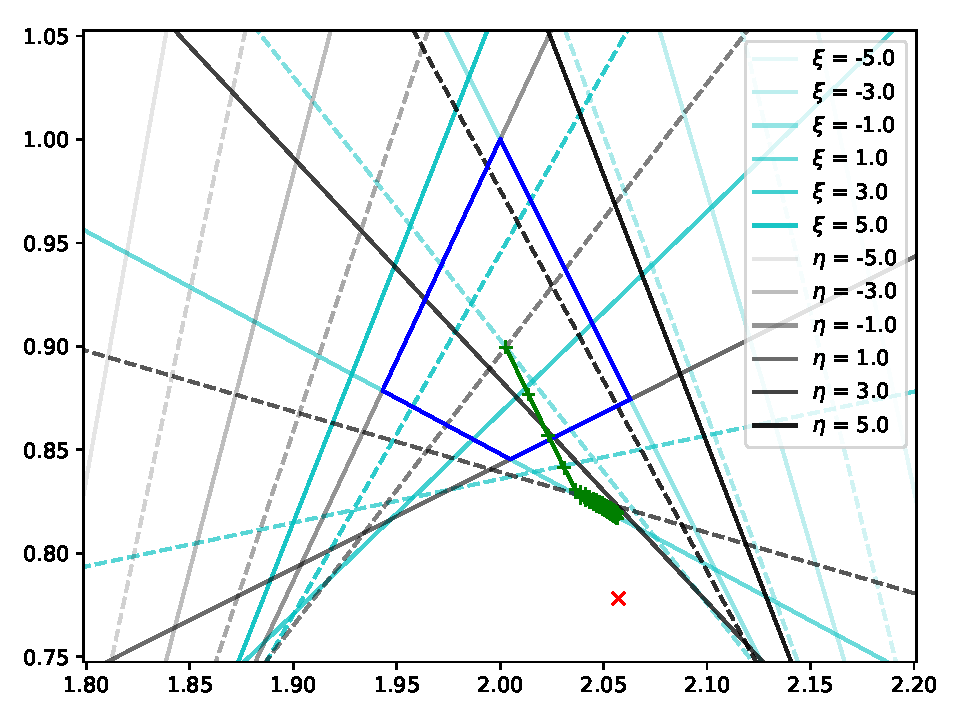
\includegraphics[width=.9\textwidth]{./coordmap.pdf}
  \caption{A failed case of the $(x,y)$-to-$(\xi,\eta)$ map which might occur in extrapolations.}
  \label{coordmap}
\end{figure}
%

%
It is an open problem to design an oscillation measure requiring no extrapolations.
%
In current work, we tried the following surface integral of value jumps
$$
\oint_{\partial E_j} \qty(u^h_{j}-u^h_{j'})^2,\quad
j'\in\text{ neighbors of } E_j,
$$
which gives reasonable results in ordinary tests.
%
Further tests on more challenging problems are still in progress.

\section{Results}
In this section, the effectiveness of the artificial viscosity proposed in the previous section is demonstrated by some standard test cases.
%
For one-dimensional problems, the computational domain is divided into $100$ elements uniformly.
%

%
A fifth-order ($P=4$) FR scheme using the $g_2$ correction function from \cite{Huynh_2007}, which is equivalent to a DG SEM scheme of the same order of accuracy, is used for spatial discretization.
%
The resulting ODE system is solved by an explicit three-stage third-order strong stability preserving Runge--Kutta method \cite{Gottlieb_2001}.

\subsection{Shock Tube Problems}
Riemann problems, as well as their exact and approximate solvers, play a pivot role in the development of CFD schemes \cite{Toro_2009}.
Among the infinite number of Riemann problems of the 1D Euler system, the Sod problem with the initial condition
\begin{equation}
\mqty[\rho & u & p]_{t=0}
=
\begin{cases}
\mqty[1 & 0 & 1], &x<0,\\
\mqty[0.125 & 0 & 0.1], &x>0,\\
\end{cases}
\end{equation}
and the Lax problem in with the initial condition
\begin{equation}
\mqty[\rho & u & p]_{t=0}
=
\begin{cases}
\mqty[0.445 & 0.698 & 3.528], &x<0,\\
\mqty[0.5 & 0 & 0.571], &x>0,\\
\end{cases}
\end{equation}
are two of the most famous ones that are frequently used for testing shock capturing techniques.

Figure \ref{fig:sod} and \ref{fig:lax} gives the solution (the \emph{Actual} curves) of these two problems at the moment ($t=0.5$ for Sod, $t=0.3$ for Lax) and the viscosity distributions for each characteristic variables at all time steps.
%
The \emph{Expect} curves in these figures are the exact solutions obtained from analytical procedures.
\begin{figure}[H]
  \centering
  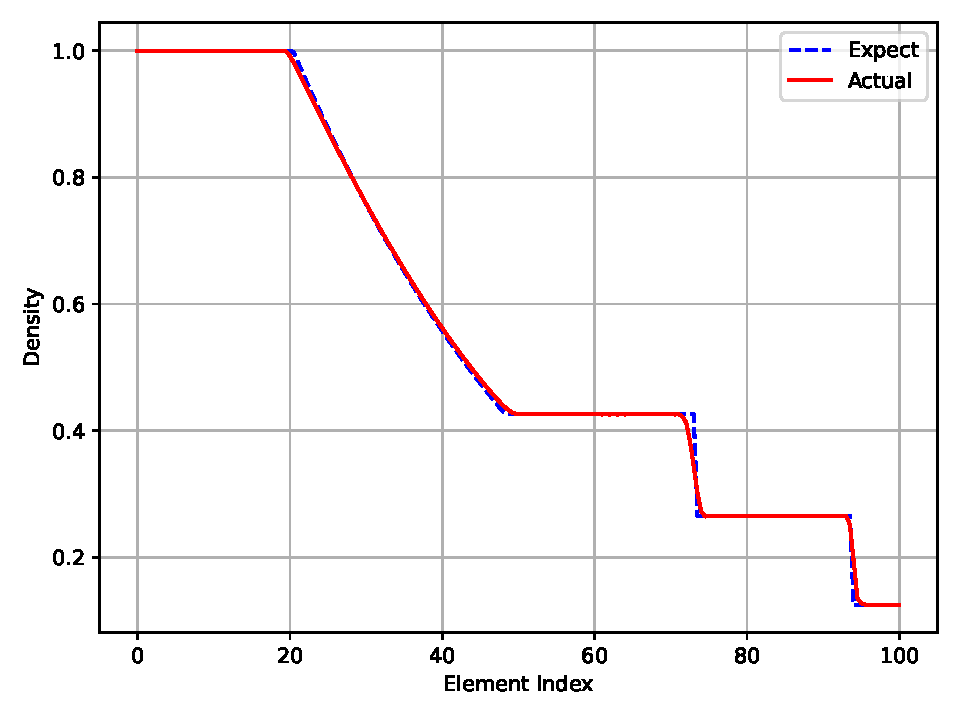
\includegraphics[width=.49\textwidth]{./sod/Frame100.pdf}
  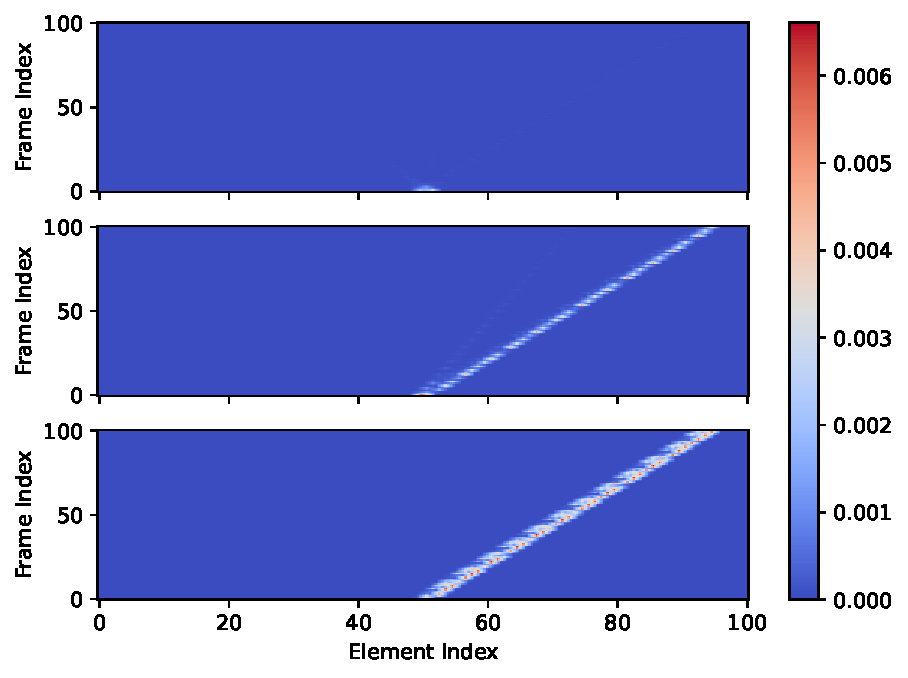
\includegraphics[width=.49\textwidth]{./sod/Viscosity.pdf}
  \caption{Solution and viscosity distribution of the Sod problem.}
  \label{fig:sod}
\end{figure}

\begin{figure}[H]
  \centering
  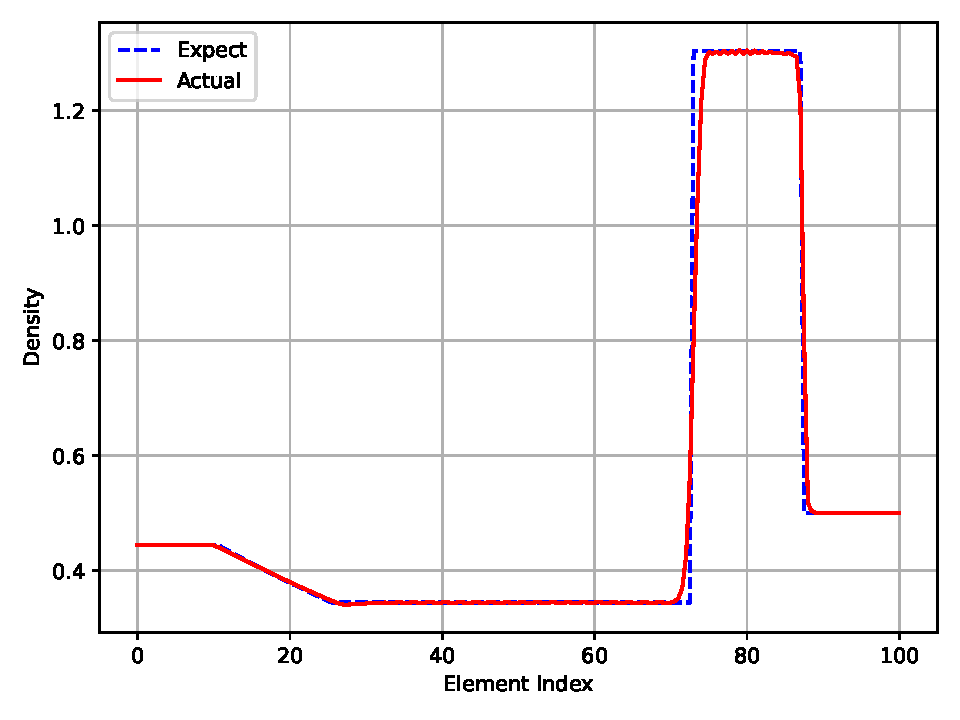
\includegraphics[width=.49\textwidth]{./lax/Frame100.pdf}
  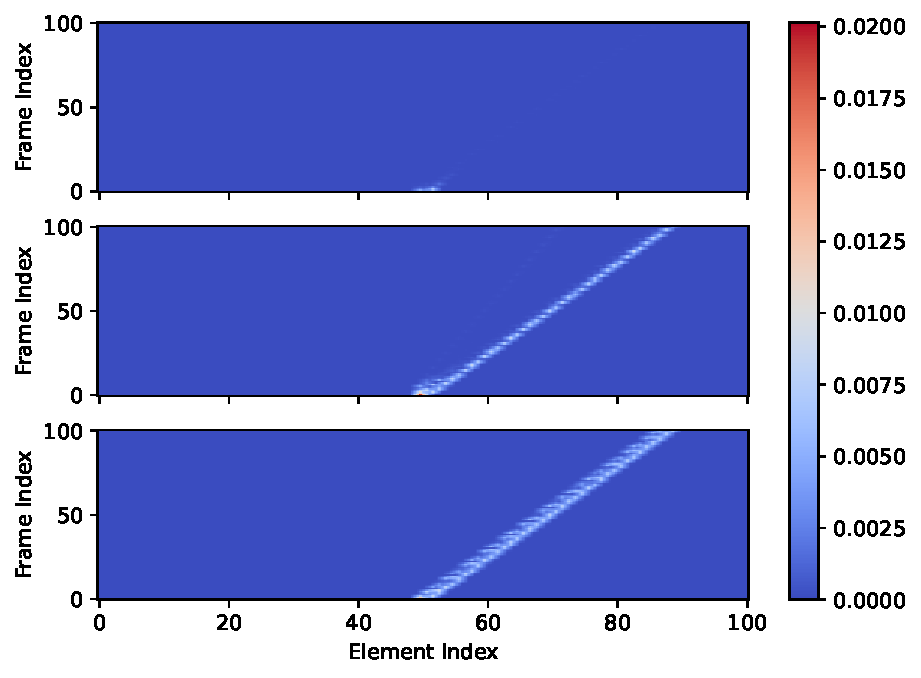
\includegraphics[width=.49\textwidth]{./lax/Viscosity.pdf}
  \caption{Solution and viscosity distribution of the Lax problem.}
  \label{fig:lax}
\end{figure}

\subsection{The Shu--Osher Problem}\label{sec:shu_osher}

The Shu--Osher problem is designed to mimic the interaction of a running shock with a standing isentropic wave \cite{Shu_1989}.

The computational domain is $x\in[0, 10]$ with two no-reflection conditions applied at the left and right boundaries.
The time range of interest is $t\in[0, 1.8]$ with the initial condition set to be
\begin{equation}
\mqty[\rho & u & p]_{t=0}
=
\begin{cases}
\mqty[3.857143 & 2.629369 & 10.33333], &x\in[0,1);\\
\mqty[1+0.2\sin(5x) & 0 & 1], &x\in(1,10].
\end{cases}
\end{equation}

Figure \ref{fig:shu_osher} gives the solution (the \emph{Actual} curve) of this problem at the final ($t=1.8$) moment and the viscosity distribution for each characteristic variables at all time steps.
The \emph{Expect} curve in this figure is the approximate solution given by the same FR scheme with a $p$-weighted limiter \cite{Li_2020} on a finer mesh (200 elements).
\begin{figure}[H]
  \centering
  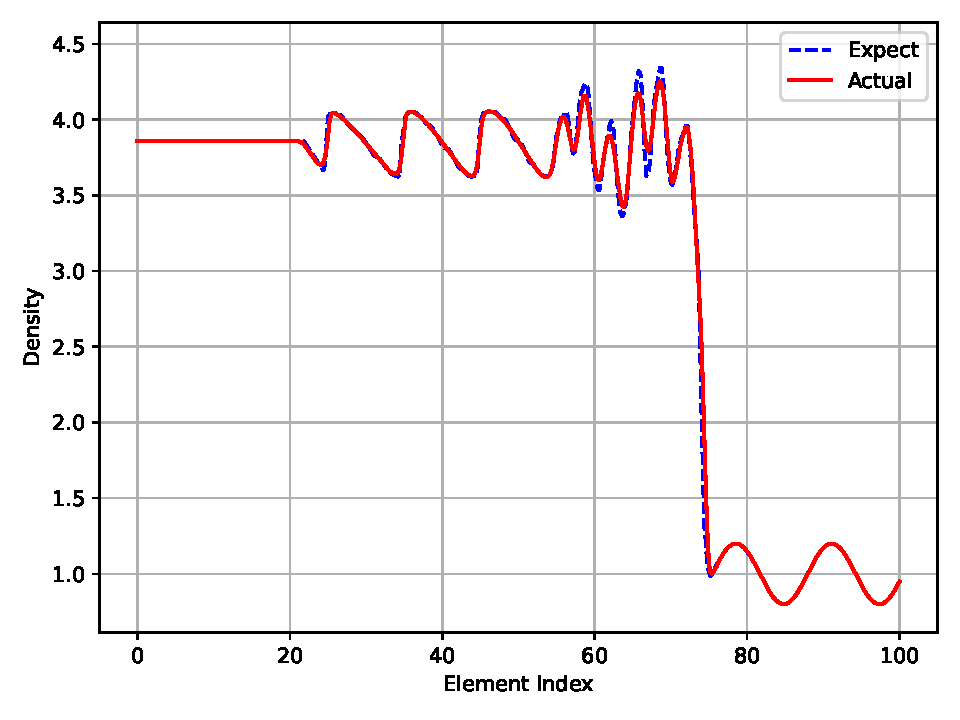
\includegraphics[width=.49\textwidth]{./shu_osher/final/Frame100.pdf}
  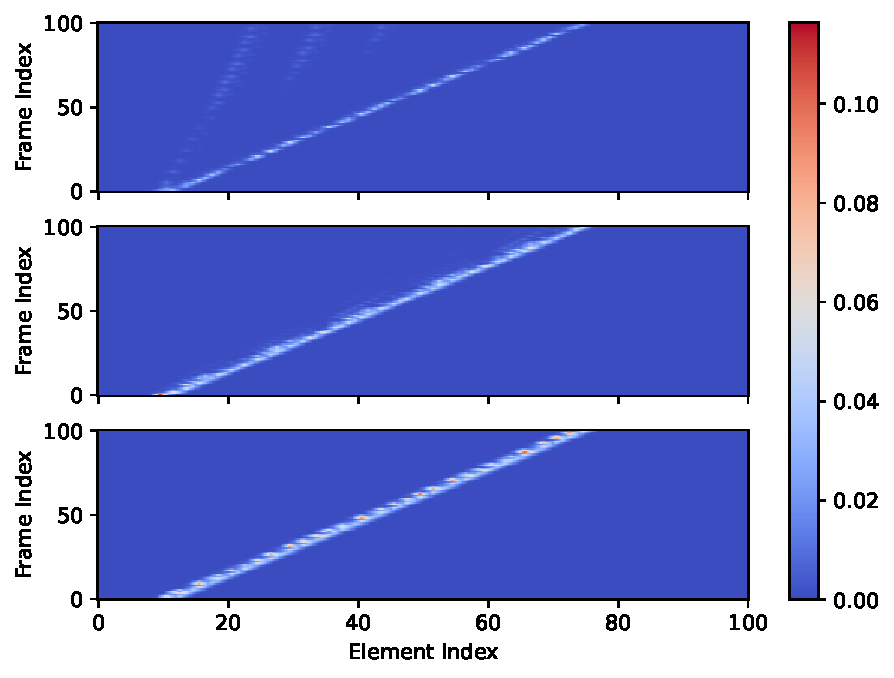
\includegraphics[width=.49\textwidth]{./shu_osher/final/Viscosity.pdf}
  \caption{Solution and viscosity distribution of the Shu--Osher problem.}
  \label{fig:shu_osher}
\end{figure}

\section{Conclusions}
The standard cases for testing shock capturing methods show that the proposed artificial viscosity is sufficiently large for suppressing numerical oscillations near physical discontinuities, such as shocks and contacts, while keeps negligible in other regions for maintaining the high-order accuracy of the DG or FR solution.

%%%% BIBLIOGRAPHY
\bibspacing=\dimen 100
\bibliographystyle{unsrt}
\bibliography{biblio}

\end{document}
